\documentclass[12pt,twoside]{article}
\usepackage{jmlda}
%\NOREVIEWERNOTES
\title
%    [Образец оформления статьи для публикации] % Краткое название; не нужно, если полное название влезает в~колонтитул
    {Определение местоположения по сигналам акселерометра}
\author
%    [] % список авторов для колонтитула; не нужен, если основной список влезает в колонтитул
    {Макаров~М.\,В.} % основной список авторов, выводимый в оглавление
%    [] % список авторов, выводимый в заголовок; не нужен, если он не отличается от основного
%\thanks
%    {Работа выполнена при финансовой поддержке РФФИ, проект \No\,00-00-00000.
%   Научный руководитель:  Стрижов~В.\,В.
%   Задачу поставил:  Эксперт~И.\,О.
%    Консультант:  Консультант~И.\,О.}
%\email
%    {author@site.ru}
%\organization
%    {$^1$Организация; $^2$Организация}
\abstract
    {Мы рассматриваем задача определения местоположения человека по данным акселерометра телефона и другим вспомогательным данным. 
    Уже существуют некоторые методы решения данной задачи \cite{journals/corr/abs-1712-09004}.
    В данной статье акцент делается на использовании дополнительной информации, например сигналов гироскопа или магнетометра, 
    для повышения точности. 
%\bigskip
%\textbf{Ключевые слова}: \emph {ключевое слово, ключевое слово,
%еще ключевые слова}.
}

\begin{document}
\maketitle
%\linenumbers

\section{Введение}
В данной работе рассматривается задача определения местоположения человека по данным акселерометра его телефона. Данная задача актуальна как часть
более общей проблемы определения местоположения. Поскольку акселерометры энергоэффективны и не требуют для работы наличие внешних устройств, таких как спутник или радиоточка, точные методы решения этой задачи востребованы.
    
В силу того, что акселерометры, использующиеся в мобильных устройствах, неточны, н
наивное решение поставленной задачи путём двойного интегрирования даёт путь, значительно отклоняющийся от истинной траектории.
В \cite{journals/corr/abs-1712-09004} эта проблема решается использованием информации о том, где находится телефон во время 
перемещения человека.

Местоположение также можно определить, используя данные других датчиков, таких как магнитометр \cite{6987239} и гироскоп \cite{s18051391}.

В данной работе сравниваются различные модели для регресии скорректированных векторов скорости, для последующего определения траектории согласно схеме, используемой в \cite{journals/corr/abs-1712-09004}. Используются данные акселерометра и гироскопа.


\section{Постановка задачи}
Данные с датчиков представляются в виде временного ряда 
\[
\mathbf{s} = \{ (\mathbf{c}(t), \mathbf{r}(t)) | t \in T \} \in {\mathbb{R}^{6 \times T}} = \mathbb{X}, \label{eq:s} \tag{*}
\]
составленного из показаний акселерометра и гироскопа по трём координатам, 
где 
$T = \{ t_i | i \in \mathcal{I} \}$, $\mathcal{I} = \{1, \ldots, m\}$ --- множество моментов в которые проводились измерения. 
Аналогично, ряд истинных положений объекта имеет вид $\mathbf{y} \in {\mathbb{R}^{3 \times T}} = \mathbb{Y}$.
Обозначим через $\mathbf{X} = \{ \mathbf{s}_i | i \in \mathcal{I} \} $ матрицу всех рядов выборки, 
а через $\mathbf{y} = \{ \mathbf{y}_i | i \in \mathcal{I} \}$ --- матрицу положений объекта в соответствующие моменты времени.

Предпологается, что 
в момент времени $t_1$ базис системы отсчёта объекта совпадает с системой отсчёта, относительно которой происходят измерения перемещения, 
погрешности измерений $\mathbf{c}_i(t), \mathbf{r}_i(t), \mathbf{b}_i(t)$ независимы и имеют нулевое матожидание, 
 каждый элемент выборки был получен при фиксированном расположении смартфона на теле человека --- в сумке, в руке, на теле или на ноге 
    --- соответственно классы $ P = \{0, 1, 2, 3 \} $.


Требуется найти такую модель 
$$ 
\mathbf{f}: \mathbb{X} \rightarrow \mathbb{Y}, \quad \mathbf{f}(\mathbf{s}) = \hat{\mathbf{y}} 
$$
что среднеквадратичная функция ошибки 
$$
    S(\hat{\mathbf{y}}, \mathbf{y}) = \frac{1}{|I|} \sum\limits_{i \in \mathcal{I}}
     \sum\limits_{t \in T} || \mathbf{y}_i(t) - \hat{\mathbf{y}}_i(t) ||^2
$$ 
минимальна.

В данной работе рассматриваются каскадные модели следующего вида:
на первом уровне 
модель $g: \mathbb{X} \rightarrow P, g(\mathbf{s}) = p$ определяет, к какому классу расположения относится данная траектория. После чего
модель $\mathbf{f}_p(\mathbf{s}) = \hat{\mathbf{v}} $ даёт оценку истинных векторов скорости. Наконец, скорости $\tilde{\mathbf{v}}$ интегрируются для получения оценки $\hat{\mathbf{y}}$.

%Таким образом, определяя $\tilde{f}(s) = I(f_{g(M(s))}(M(s)))$ формальная постановка задачи такова:
%$$
%    \mathbf{f}^* = \argmin_{g, f_1, \ldots, f_3 } S(\tilde{f}(\mathbf{X}), \mathbf{y})
%$$

\section{Базовый алгоритм}

В качестве базового алгоритма рассматривается численное интегрирование сигнала акселерометра 
без фильтрации сигнала в предположении, что ориентация смартфона не меняется во времени. Cм. $\mathbf{s}$ в  \eqref{eq:s} 
$$
    \mathbf{f}(\mathbf{s})(t_i) = \sum\limits_{j=2}^{i} \left(
    \sum\limits_{k=2}^{j - 1} \mathbf{c}_k (t_k - t_{k - 1}) + \frac{1}{2}\mathbf{c}_j (t_j - t_{j - 1})
    \right) (t_j - t_{j - 1}), \quad \mathbf{f}(\mathbf{s})(t_1) = 0.
$$

Как описано, например, в \cite{journals/corr/abs-1712-09004}, интегрирование даёт неточный результат на шумном входе.

\section{Базовый эксперимент}

Для получения матрицы признаков $X$ предварительно из данных удаляются высоко-частотные шумы с помощью сглаживания Гаусса. Полученные линейные и угловые скорости уже преобразуются в вектор признаков.

В качестве модели рассматривается каскадная регрессия, состоящая из классификатора положения датчиков и семейства регрессоров на каждый из классов, как в ~\cite{journals/corr/abs-1712-09004}. 

По матрице признаков $X$ классификатор определяет, какому расположению датчиков (в руке, на ноге, на поясе, в сумке) соответствует данное описание, т.е. решает задачу многоклассовой классификации с 4 классами.

После этого для каждого класса на тренировочной выборке обучается свой регрессор, который выдает скорости движения пешехода для каждого временного блока. Полученные скорости содержат ошибку, связанную с неточностями инерционных датчиков, поэтому далее для этих скоростей находится смещение (по предположению низко-частотное) из следующей задачи минимизации:

\[\min_{\{x^1_I, x^51_I,\dots\}}V_{bias}=
\min_{\{x^1_I, x^51_I,\dots\}}\sum_{f \in F_2}\|v_C^F-v_R^f\|+
\lambda\sum_{f \in F_1}\|x^f_I\|^2,\]
\[v_C^f = R_{SW}^f\sum_{f'=1}^f R_{WI}^{f'}(a_I^{f'}+x_I^{f'}),\]
где $f$ - единица блока выборки, $F$ - блок выборки, $v_C^F$ - скорректированное значение скорости, $v_R^f$ - предсказанное значение скорости, $I$ - система координат устройства, $W$ - глобальная система координат, $S$ - IMU-стабилизированная система координат, $R_{AB}$ - матрица перехода из системы координат $B$ в систему координат $A$.

Также для каждого класса создается регрессор, предсказывающий угловые скорости пешехода в каждом временном блоке. 

На контрольной выборке для классификатора и каждого регрессора подбираются оптимальные значения гиперпараметров.

По полученным значениям скоростей восстанавливается траектория пешехода.


Для эксперимента используется часть данных, собранных в статье, описывающей алгоритм RIDI~\cite{journals/corr/abs-1712-09004}. Эти данные были получены с помощью инерционных датчиков, расположенных в смартфонах в нескольких случаях: когда смартфон располагался на поясе, в руке, на ноге или в сумке. Выборки содержат различные траектории длиной в 100 минут и частотой сигнала 200 Гц. В качестве объекта рассматривается положение в определенный момент времени $i$. Признаками объекта являются угловые скорости и линейные ускорения в стабилизированной системе координат датчиков в моменты времени $i-window\_size, \dots, i$, где $window\_size$ - размер окна (равен 200). Целевыми переменными являются метки классов, характеризующие то, в каком положении находился смартфон при получении определенных данных, а также скорости в данный момент времени $i$, которые вычисляются через координаты пешехода и прошедшее время. По полученным данным после уточнения скоростей с помощью оптимизации функции  $V_{bias}$ строится предсказанная траектория пешехода.

Цель эксперимента: подобрать такие модели и их параметры, что предсказанная траектория пешехода будет наиболее близкой к истинной.


Формально алгоритм описывается следующим образом: 

\begin{algorithmic}[1]
    \REQUIRE $X, Y_{class}, Y, X_{test}$
    \STATE $initialize ~ classifier\_options$
    \STATE $classifier = Classifier(classifier\_options);$
    \STATE $classifier.fit(X, Y_{class})$
    \FOR {$cls ~ in ~ classes$:}
    \STATE $initialize ~ regressor\_cls\_optons$
    \STATE $regressor\_cls = Regressor(regressor\_cls\_optons)$
    \STATE $regressor\_cls.fit(X[X[ind] \in cls], Y)[Y[ind] \in cls])$
    \ENDFOR
    \STATE $Y_{test-class} = classifier.predict(X_{test})$
    \FOR {$cls ~ in ~ classes$:}
    \STATE $Velocity\_cls = regressor\_cls.predict(X_{test}
    [Velocity\_class[ind] == cls]$
    \STATE $x^1_I, x^51_I,\dots = \argmin_{\{x^1_I, x^51_I,\dots\}}V_{bias}\_cls$
    \STATE $Velocity\_cls = R_{SW}^f\sum_{f'=1}^f R_{WI}^{f'}(a_I^{f'}+x_I^{f'})$
    \STATE $Trajectory\_cls$ recovery depending on $Velocity\_cls$
    \ENDFOR
    \RETURN $Full\_trajectory$
\end{algorithmic}

\section{Рассмотрение моделей}

Вся выборка была разбита на обучающую и тестовую, причём данные в тестовой выборке были сняты с других людей.
Для моделей производился подбор гиперпараметров с помощью кросс-валидации по тренировочной выборке, а также измерялось их качество на тестовой выборке.

\subsection{Метод ближайших соседей}
В качестве первого класса моделей рассматривался метод ближайших соседей. Подбирались следующие параметры: число соседей, метрика и функция весов.

\begin{figure}[H]
    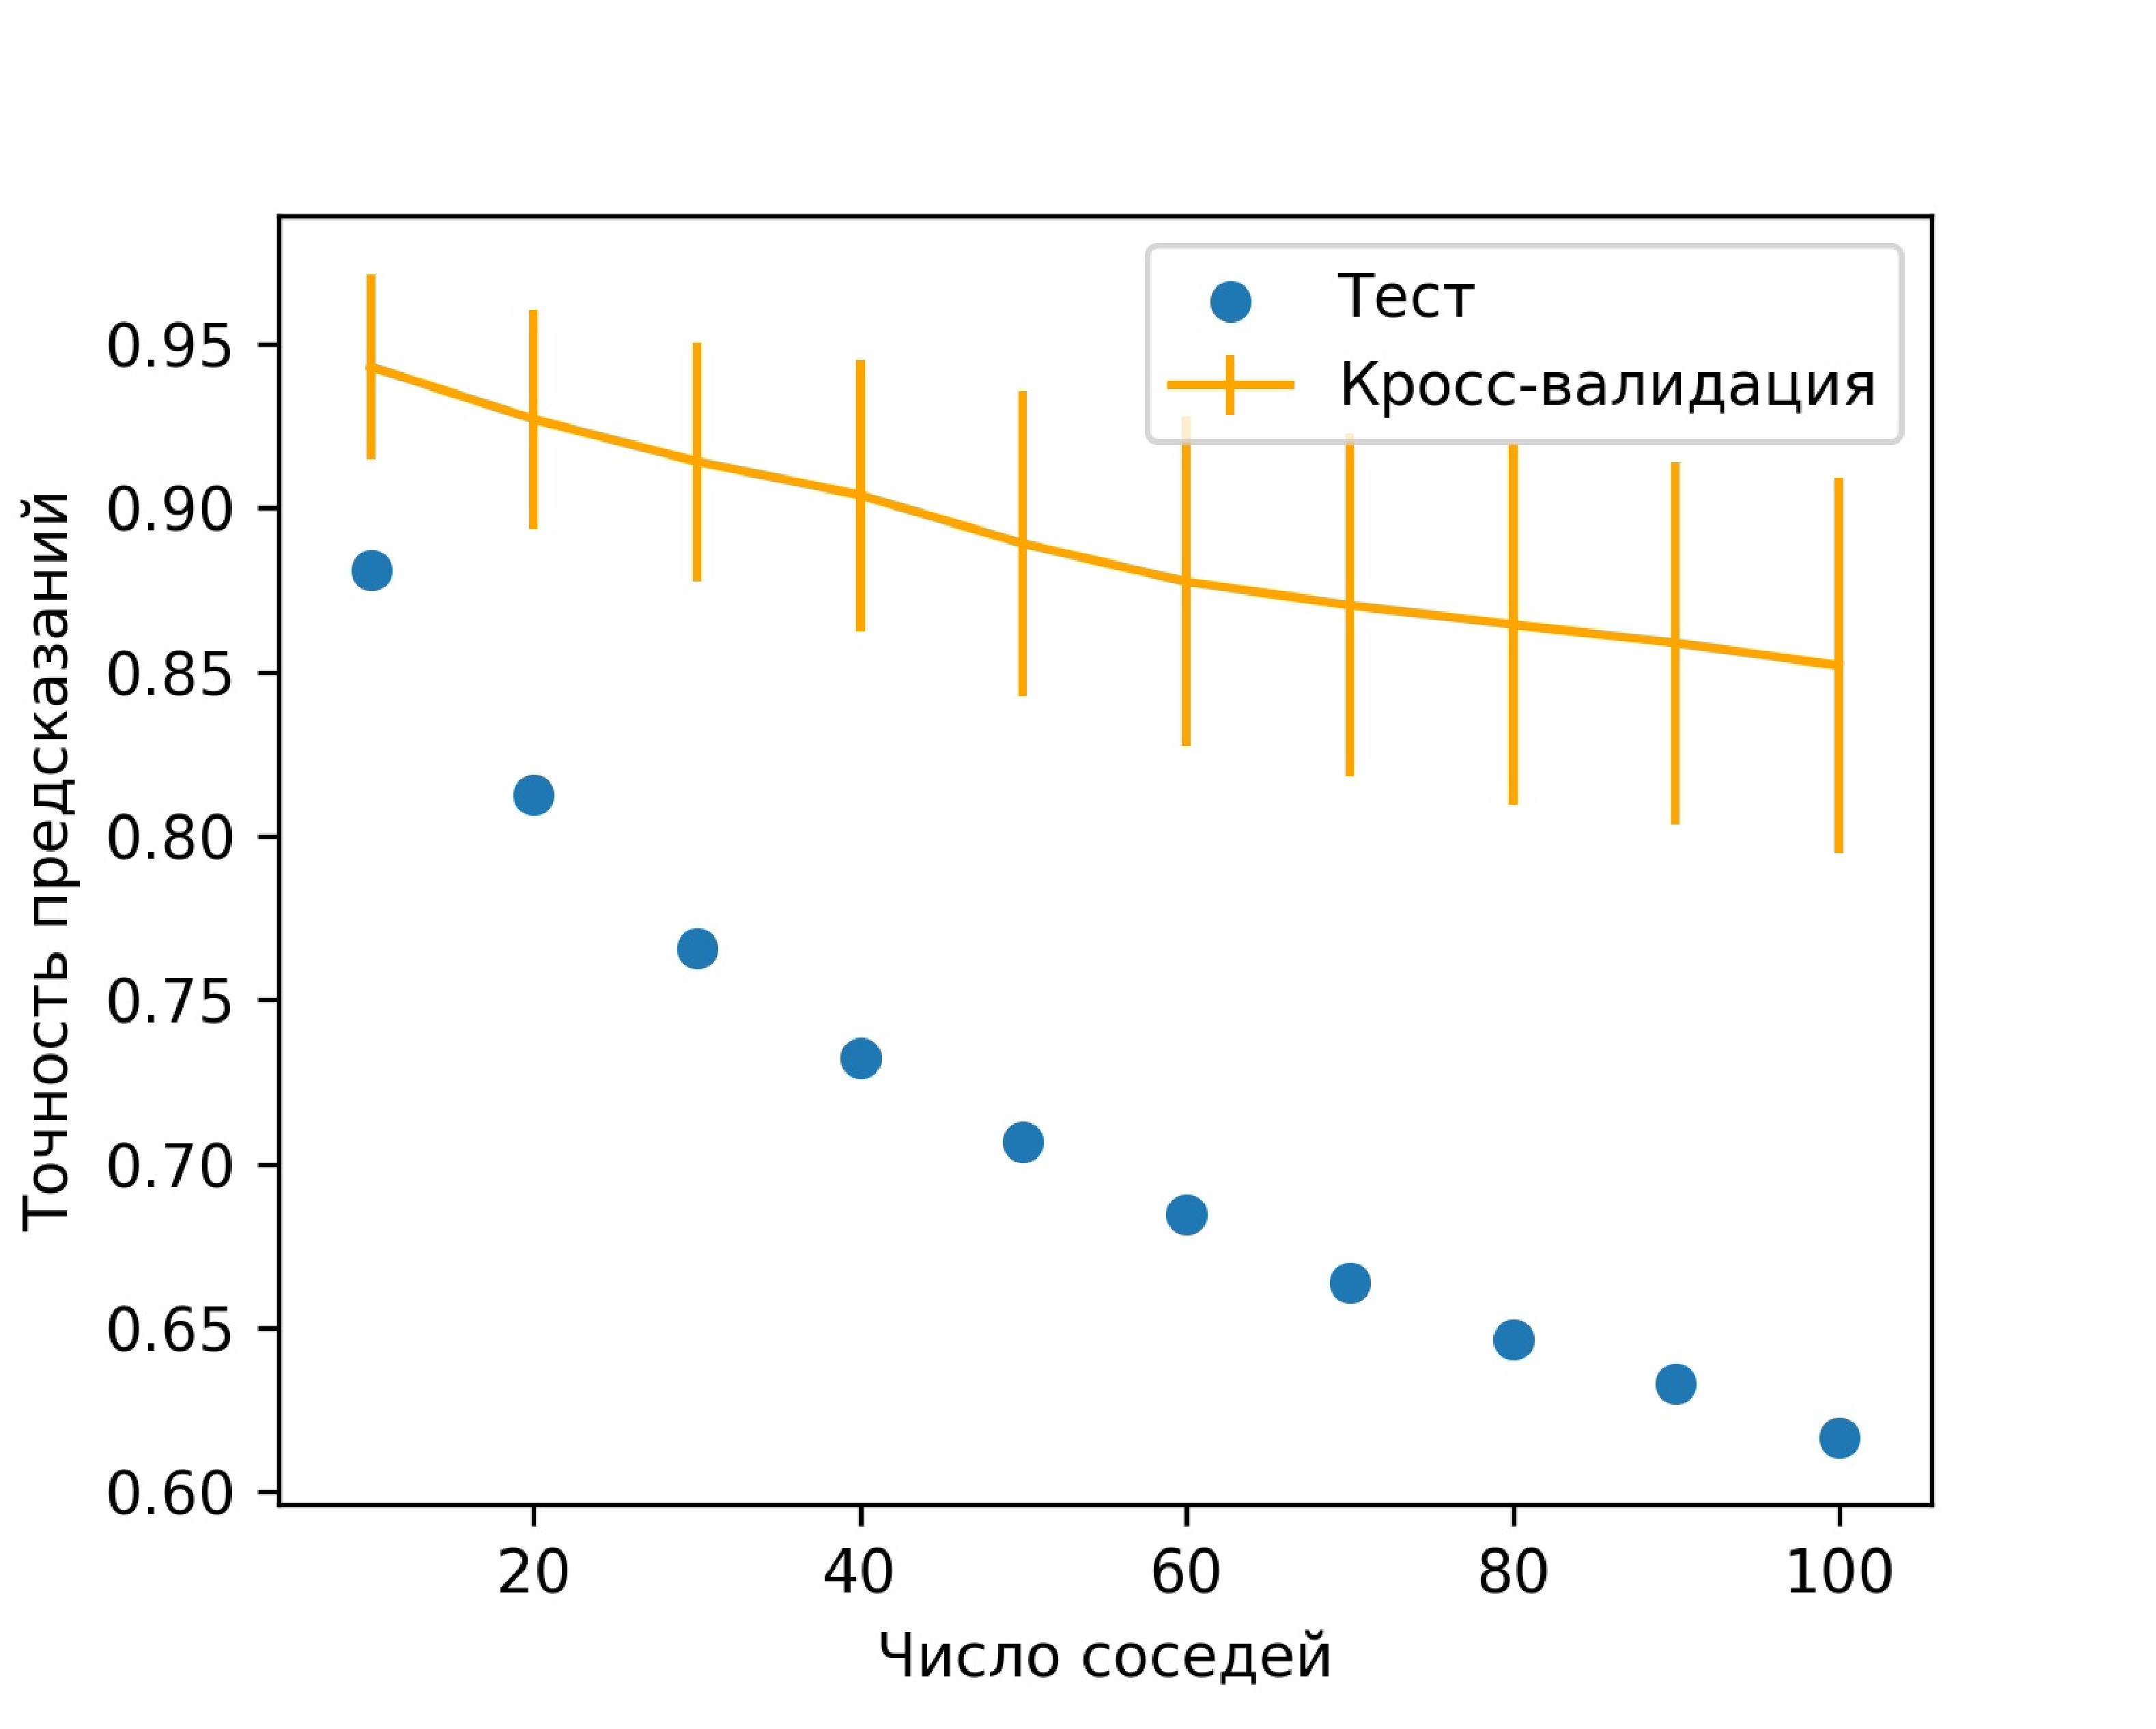
\includegraphics[scale=0.15]{charts/knn.eps}
    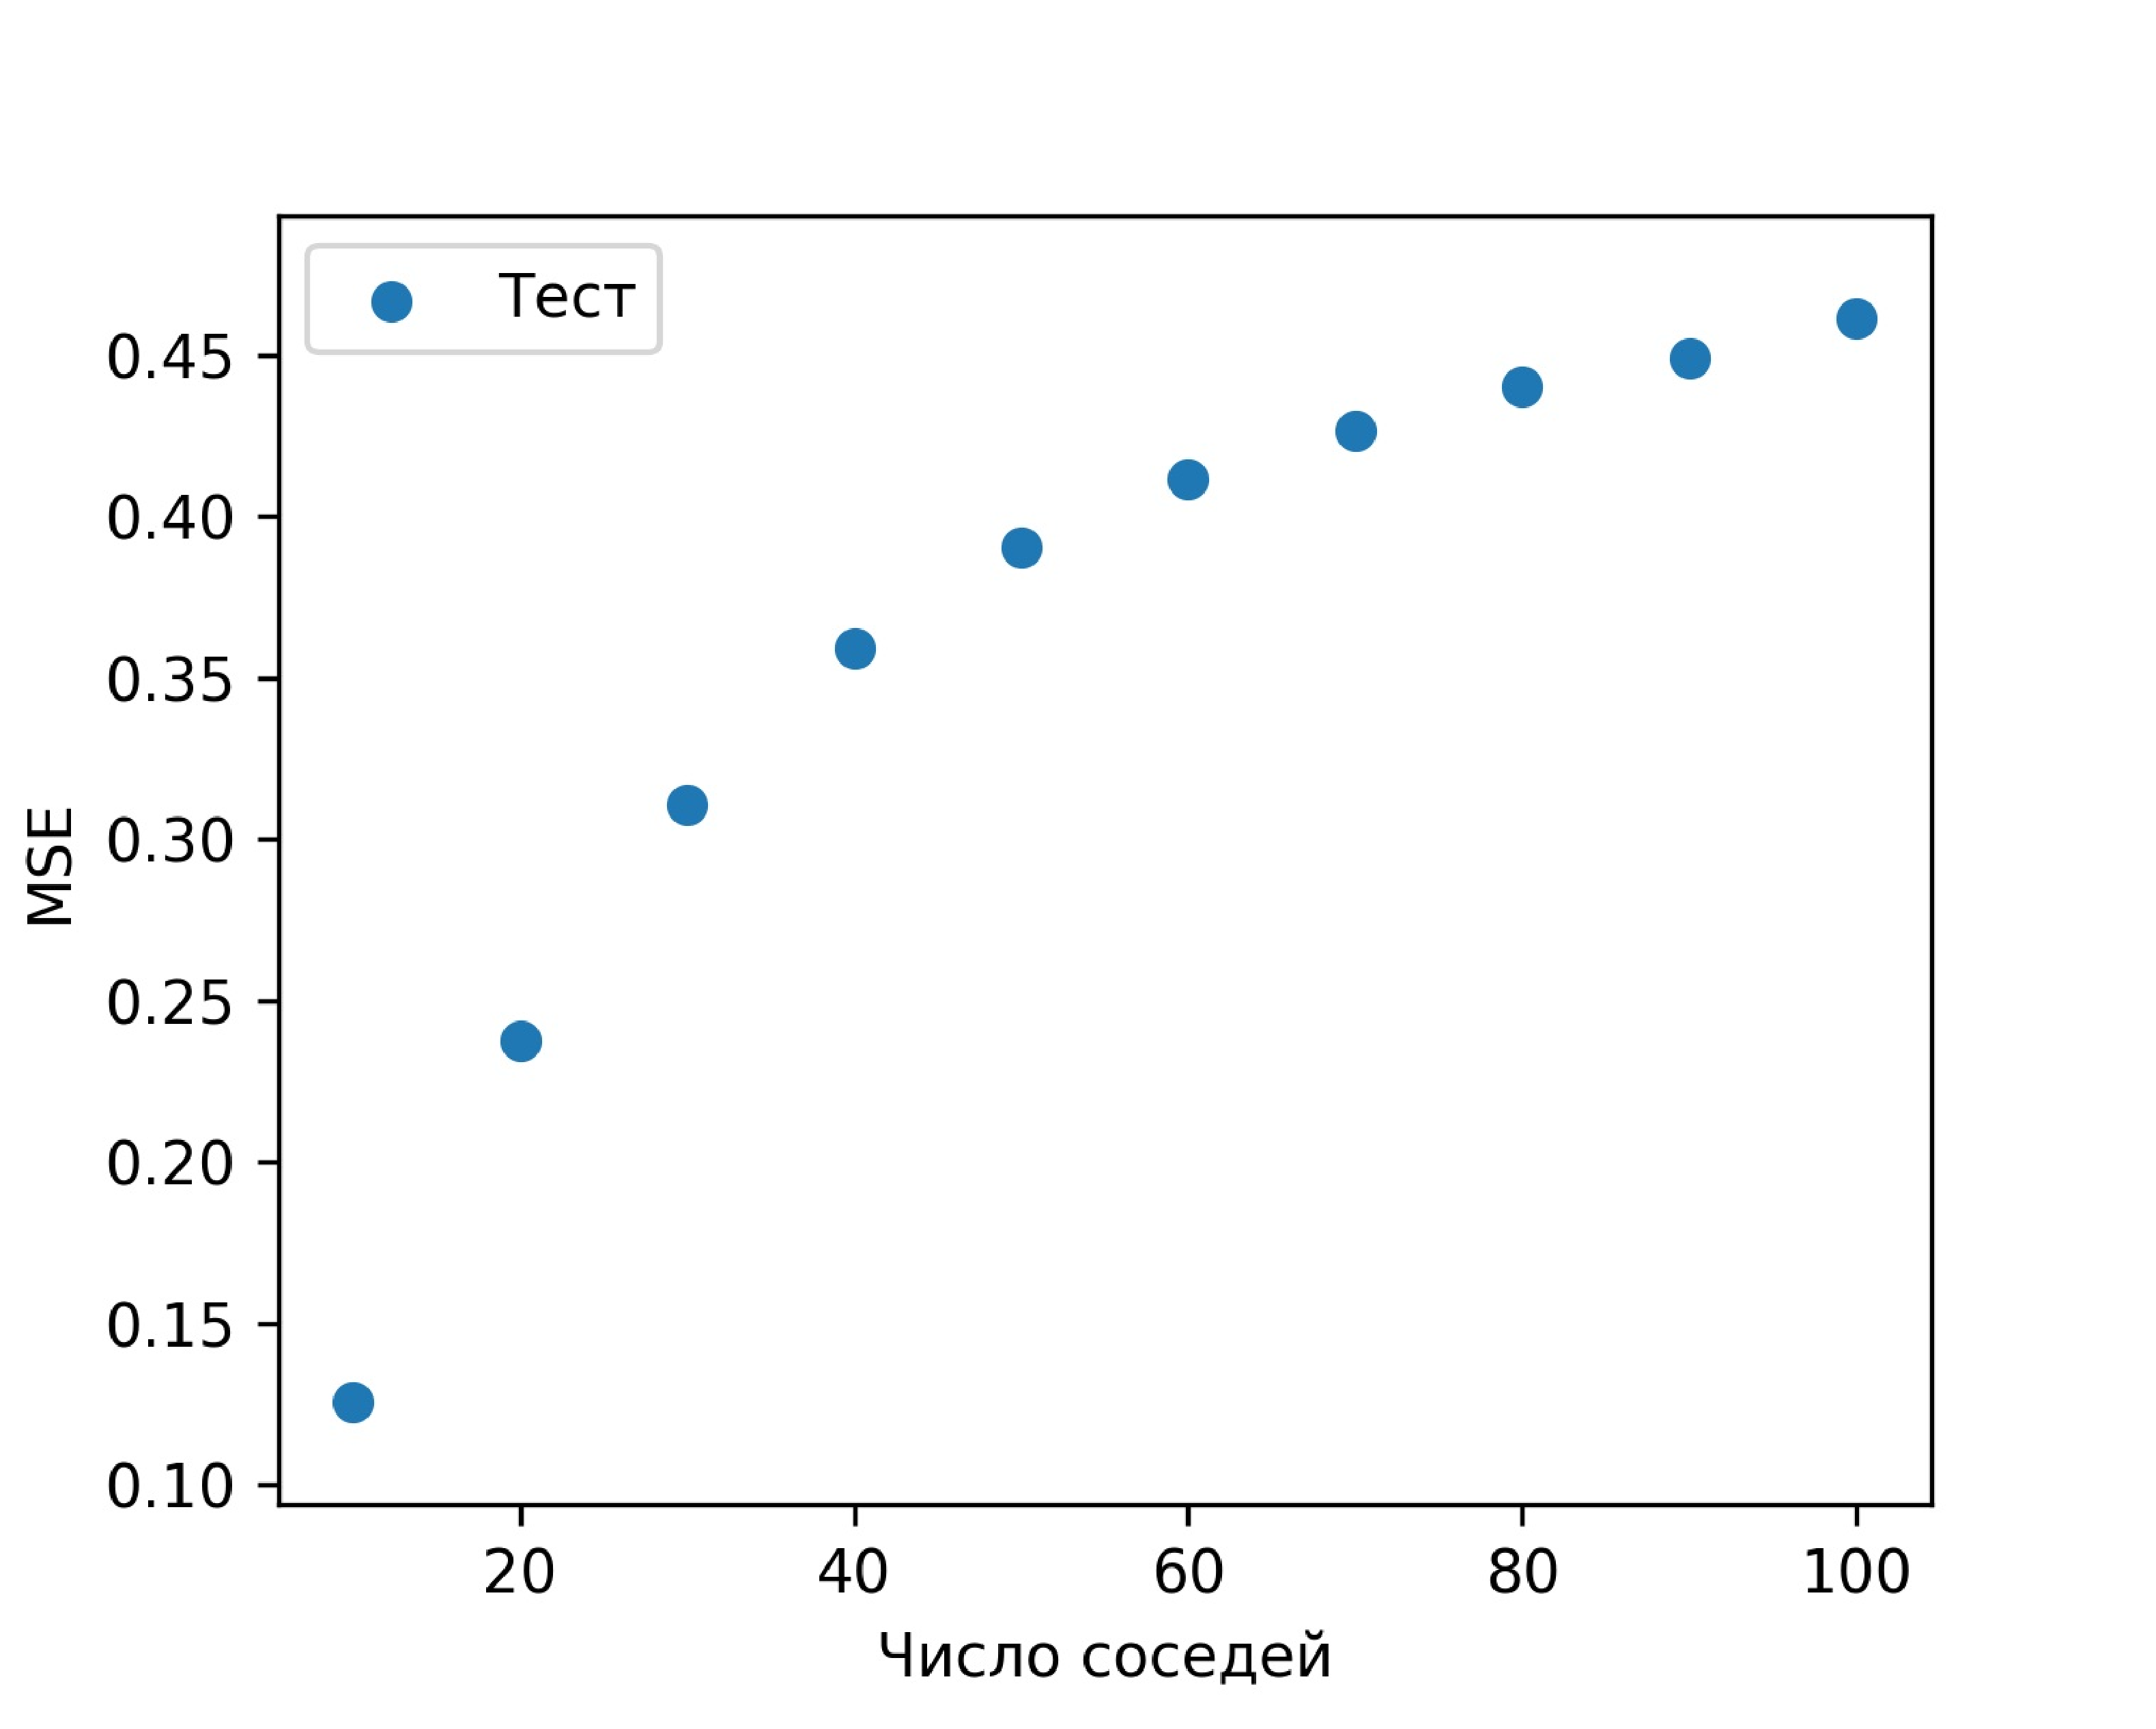
\includegraphics[scale=0.15]{charts/knn_mse.eps}
    \centering
    \caption{Точность предсказания класса и ошибка на тесте, kNN}
    %\label{fig:image}
\end{figure}

В итоге наилучшей метрикой оказалась $l1$, а наилучшей функцией весов оказалось расстояние.

\subsection{Свёрточные нейронные сети}

Вторым рассмотренным классом классификаторов были свёрточные нейронные сети. Исторически они использовались для задачи распознавания действий человека (Human Activity Recognition) \cite{7379395}. Архитектура сети была выбрана, основываясь на \cite{DBLP:journals/corr/abs-1809-04356} \cite{7870510}.

\begin{tabular}{l l l}
    Тип & Слой & Параметры \\
    \hline
    A1 & Свёрточный слой & Выходное число каналов --- 12, длина ядра --- 7 \\
    A2 & Average pooling & Длина --- 3\\
    B  & Полносвязный слой & Число нейронов --- 16\\
    C1 & Softmax слой & Число классов --- 4\\
    C2 & Полносвязный слой без активации & Число нейронов --- 1
\end{tabular}

Рассматривались архитектуры следующего вида:
\begin{itemize}
    \item От 1 до 3 пар слоёв A1, A2.
    \item От 0 до 2 слоёв B.
    \item Слой C1 для классификатора или слой С2 для регрессоров.
\end{itemize}
В качестве функции активации использовалась ReLU.

Каждая из них обучалась 200 эпох на обучающих данных под контролем валидационной выборки. Две наилучшие из них --- с 3 свёрточными и 2 полносвязными и с 2 свёрточными и 2 полносвязными слоями. Также хорошие результаты на классификации показала архитектура с одним свёрточным и одним полносвязным слоями.

\begin{figure}[H]
    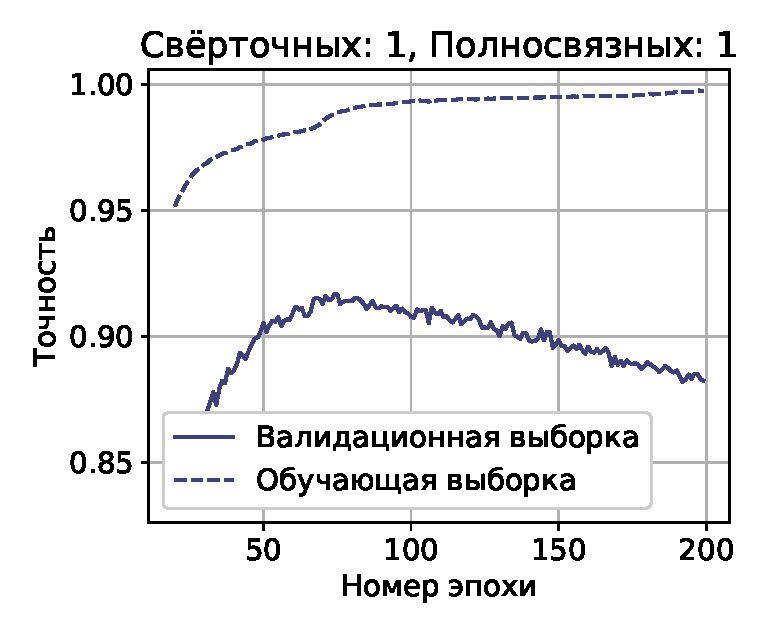
\includegraphics[scale=0.45]{charts/cnn11.eps}
    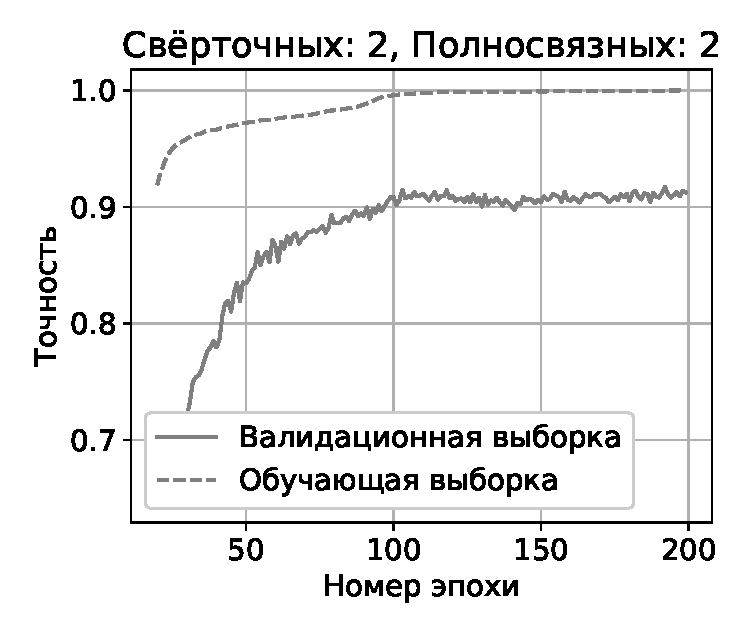
\includegraphics[scale=0.45]{charts/cnn22.eps}
    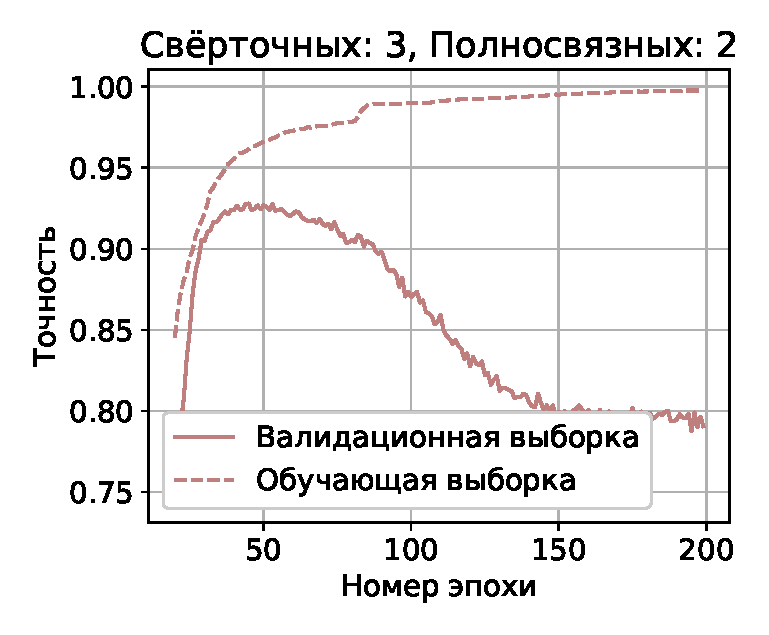
\includegraphics[scale=0.45]{charts/cnn32.eps}
    \centering
    \caption{Точность предсказания, CNN}
\end{figure}

\begin{figure}[H]
    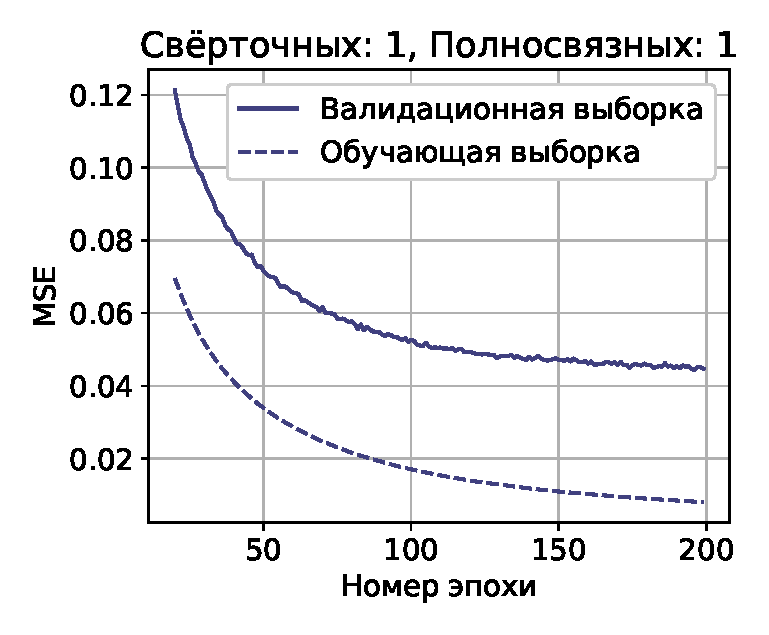
\includegraphics[scale=0.44]{charts/cnn11_mse.eps}
    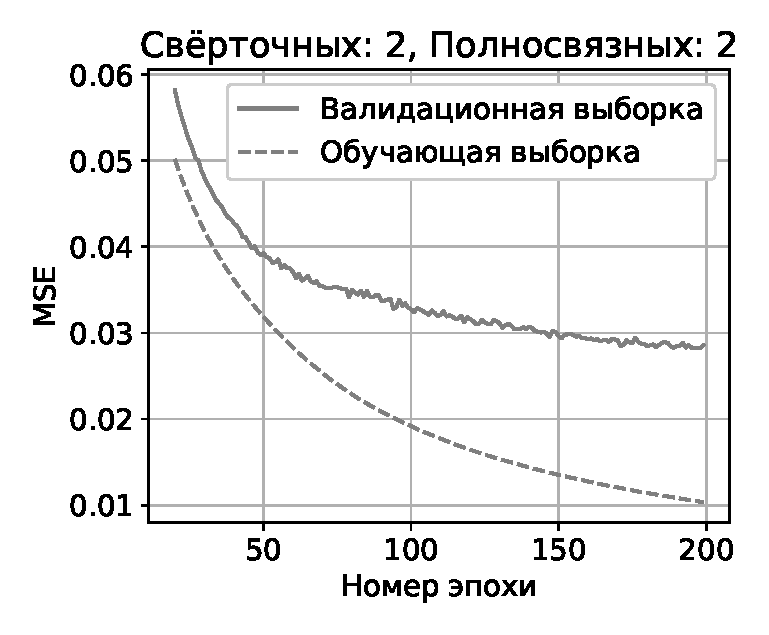
\includegraphics[scale=0.44]{charts/cnn22_mse.eps}
    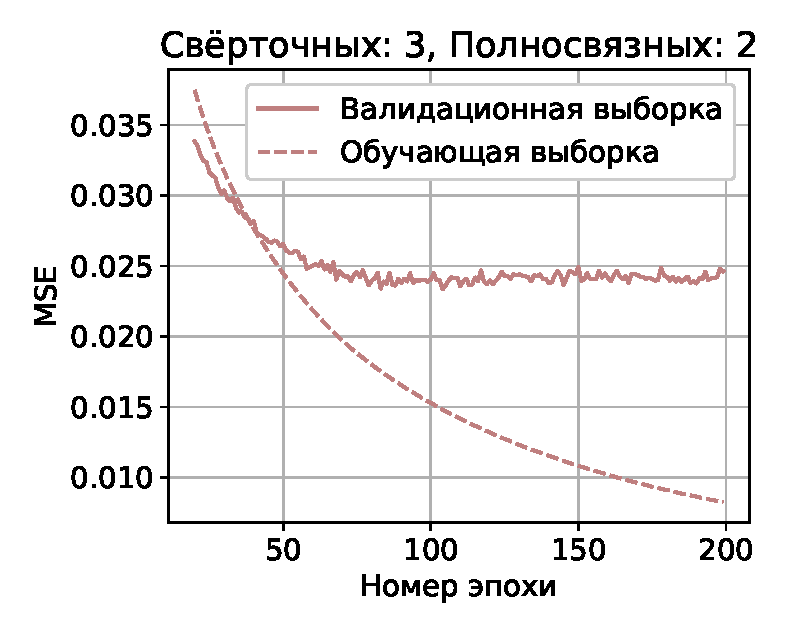
\includegraphics[scale=0.44]{charts/cnn32_mse.eps}
    \centering
    \caption{Ошибка регрессии, усреднённая по классам и каналам, CNN}
\end{figure}

Наилучшую точность и наименьшую ошибку регрессии показала архитектура с 3 свёрточными и 2 полносвязными слоями --- $92.8\%$ и $0.028$ соответственно.

\section{Выводы}

Как и ожидалось, увеличение сложности модели может повысить качество на обоих уровнях каскада, как это видно для регрессии в сравнении SVM и свёрточной сети. Но, к сожалению, это так далёко не всегда, что хорошо демонстрирует метод ближайших соседей. С другой стороны, большая сложность модели также означает, что модель будет требовать больших вычислительных ресурсов, что будет означать её неприменимость для устройств с небольшими вычислительными мощностями.

\nocite{*}
\bibliographystyle{unsrt}
\bibliography{MakarovProject26}
\end{document}
